\chapter{Entropy-based measures of verbal valency}\label{chapter:entropy}

While the previous chapter has demonstrated that corpus-based transitivity ratios can serve as a useful basis for typological comparison, it is still is a relatively simple metric that captures one aspect of verbal valency. Put another way, transitivity ratio can be seen as a subset of the scope needed for a more holistic investigation into verbal valency, as it concerns only one type of verb dependent, i.e., the object, and one feature of this dependent, i.e., its presence or absence. 

This chapter undertakes to expand the scope of investigation accordingly, to cover both more verb dependent types and more features of them. Instead of performing exhaustive comparisons on each individual feature of each dependent, the focus is instead on measuring the alternations of valency frames (diathesis alternations), i.e., range of the valency frames in which a verb appears and how often it appears with them. To that end, I propose new metrics of verbal valency based on entropy, a concept from information theory that quantifies the average amount of surprisal expected from a variable, and look at whether it reflects universals of how languages structure their verbal lexicons.

% In §X, valency frame entropy conditioned on the verb is calculated to measure ; §X, ablation study to see how different aspects of valency frame encoding contribute; in §X, the reverse verb entropy conditioned on the frame is calculated as a symmetric check on the measures. 

\section{Valency frame, frequency and the efficient organization of the lexicon}

Cognitive linguists and typologists have increasingly sought to integrate the two approaches in the same functionalist research paradigm \citep{croft2016}. Among others is research that seeks to examine and explain language-internal and cross-linguistic features of human languages through the lens of communicative efficiency, at various levels including the lexicon, syntax and morphology (see \citealp{gibson2019} for a survey). 

An early example where efficiency is used to explain phenomena in human languages is the work of George Kingsley \citet{zipf1935,zipf1949}. He first studied what is now known as Zipf's law, the empirical observation of the negative correlation between word length and frequency, that ``the magnitude of words tends, on the whole, [stands] in an inverse (not necessarily proportionate) relationship to the number of occurrences'', and sought to explain it through the principle of least effort.

Frequency is a particularly frequent lens through which the lexicon is examined and the correlation between frequency and other features often subjects of hypotheses. Its importance has been further underlined by psycholinguistic studies which show a consistent ``frequency effect'' for both open and closed class word \citep{segui1982,marslen-wilson1990}, where more frequently occurring words have a higher resting activation, making their lexical retrieval easier. That the most frequent lexical items are also more likely to be associated with irregularity is not surprising. This correlation between frequency and irregularity has most often been hypothesized and studied for morphology \citet{wu2019}. \citet{bybee1998} considers lexicon from a learnability perspective and postulates a trade-off in the lexical memory that ``being easier to access, they are less likely to be replaced by regular formations''. 

When it comes to verbal valency, psycholinguistic studies have also consistently shown the effect of semantic and syntactic attributes of the verb on online sentence processing \citep{shapiro1987,collina2001}. Results differ on whether subcategorization (syntactic), thematic frames (semantic) or both have an effect on lexical processing. \citet{shapiro1987} reported that RTs for lexical decisions increased as the function of the number of thematic options instead of subcategorization options. In contrast, \citet{shetreet2007} reported on an fMRI study on Hebrew speakers, shows that the number of options in terms of subcategorization and thematic frames is better correlated to activity in the cortical areas that are associated with linguistic processing, as opposed to the number of complements or thematic frames.

In the following experiments, I will test a few hypotheses between frequency metrics on the one hand and entropy metrics on the other hand and show that, regardless of the theoretical stance, how a language structures it valency system reflects trade-offs predicted by considerations of efficiency and learnability.

\section{Extracting valency frames from UD}

Besides the information about transitivity, UD annotations make available further information that are related to the morphosyntactic encoding of valency frame, including information about further dependents, word order, as well as case and adpositional markings. In the following experiments, I make use of this information for a more fine-grained characterization of the variation in valency frame encoding for different verbs using entropy-based measures.

\begin{table}
  \centering
  \begin{tabular}{ll}
    \toprule
    \textbf{UD label} & \textbf{Dependent} \\
    \midrule
    \textsc{nsubj} & nominal subject \\
    \textsc{obj} & object \\
    \textsc{csubj} & clausal subject \\
    \textsc{ccomp} & clausal complement \\
    \textsc{xcomp}   & open clausal complement \\
    \midrule
    \textsc{iobj} & indirect object \\
    \textsc{obl} & oblique nominal \\
    \textsc{expl} & expletive \\
    \textsc{advmod} & adverbial modifier \\
    \textsc{advcl} & adverbial clause modifier \\
    \bottomrule
  \end{tabular}
  \caption{UD dependent labels included in valency frame extraction}\label{tab:ud-dependent-labels}
\end{table}

To compute the entropy measures,  \textbf{valency frame encoding} information must first be extracted from the UD annotations at a token level for each verb instance. I start by determining the scope of the investigation and select a list of dependency relations in Tab.~\ref{tab:ud-dependent-labels} which categorizes different syntactic dependencies that can be attached to the verb. These include core dependents, including nominal subject, object and their clausal counterparts, as well as so-called non-core dependents, such as indirect object, adverbial modifier and expletive. \todo{justification for including non-core dependents: syntactic classification of verb using non-core information, cite previous work} It is important to note here that it is the cross-lingual taxonomy of the dependencies that serves as the cross-linguistic basis of comparison and that the name of the labels, while linguistically informed, do not affect the entropy calculation in any way.

I extract information about (1) the presence or absence of dependency relations attached to a verb token, (2) the word order information, whether specific dependents precede or follow the head verb, and (3) morphological case marking on the dependents, if any.

\todo{some concrete examples for what is to be extracted}

\section{Experiment 2: Frequency correlation with valency frame entropy}

\subsection{Experiment setup}

This experiment introduces a valency frame entropy metric, conditioned on the verb, that measures the average amount of surprisal, i.e., uncertainty, associated with the valency frame alternation for a verb, and hypothesize a positive correlation between a verb's frequency and the valency frame entropy conditioned on it that should hold across languages. In other words, the more frequent a verb is, the more information content one can expect on average from its valency frames.

A learnability perspective on the lexicon provides one motivation behind the hypothesis. Taking the view that the lexicon is acquired from linguistic experience, more exposure to and access of the more frequent words leads to higher resting activation (cf. \citealp*{bybee1998}), therefore allowing for more complexity or uncertainty being retained in the lexicon. This is analogous to the correlation between word frequency and irregularity in morphological patterns. However, whereas morphological irregularity is a purely formal feature, the choice of valency frame often entails a semantic choice as well.

If viewed from a production and comprehension perspective, the hypothesis is also potentially relevant to the Uniform Information Density (UID) hypothesis \citep{fenk1980,levy2006}, which posits that language speakers prefer a more even distribution of surprisal values across utterances in order to maximize but not overload the capacity of the communication channel. Less frequent verbs would already have high surprisal, having high entropy in the valency frames associated with it is undesirable due to channel capacity constraints. I note, however, that UID hypothesis has mostly focused on surprisal at a token/phoneme-level. This is the case for the verb in question, but the valency entropy measures aspects of the morphosyntax of the sentence instead and requires a clearer formulation of the relationship between the frames and the tokens that compose it. Nevertheless, at a high level the hypothesis here is congruent what is expected given the UID hypothesis.

Let $X_1, X_2,\ldots,X_n$ be discrete random variables where each $X_k$ represents a UD dependency relation (e.g., \textsc{nsubj}, \textsc{obj}, \ldots). These variables have corresponding sample spaces $\mathcal{X}_1, \mathcal{X}_2, \ldots, \mathcal{X}_n$, which represent the possible outcomes of each variable with regard to its presence, linearized order, and any case information. Additionally, let there be a variable $V$ that represents the choice of a verb from the lexicon $\mathcal{V}$. 

The entropy of each dependency relation given a specific verb $v \in \mathcal{V}$ quantifies the average surprisal associated with that dependency relation. It is defined as:

\begin{equation*}
  H(X_{k}|V=v)=
  -\sum\limits_{x_{k}\in{}\mathcal{X}_{k}}{P(x_{k}|V=v)\log_{2}{P(x_{k}|V=v)}}  
\end{equation*}

Here, $P(x_k | V = v)$ represents the conditional probability of the outcome $x_k$ of the dependency relation $X_k$ given that the verb variable $V$ takes on the value $v$. The entropy of $X_k$ is calculated by summing the products of these probabilities with their logarithms (base 2) taken, each corresponding to a possible outcome $x_k$.

The \textbf{valency frame entropy} is formalized as the joint entropy of the relevant UD dependency relations, i.e., number of bits needed to encode the entire valency frame. Denoted as $H_{\text{joint}}(X_1, X_2, \ldots, X_n | V = v)$, it quantifies the uncertainty associated with the combined set of random variables $X_1, X_2, \ldots, X_n$, again given a specific value $v$ for the verb variable $V$. This is defined as:

\begin{equation*}
\begin{split}
 & H_{\text{joint}}(X_1, X_2, \ldots, X_n | V=v) \\
=& -\sum\limits_{x_1\in{}\mathcal{X}_1}\cdots\sum\limits_{x_n\in{}\mathcal{X}_n}{P(x_1, x_2, \ldots,x_{n}|V=v)\log_2P(x_1, x_2, \ldots,x_n|V=v)}
\end{split}
\end{equation*}

Here, $P(x_1, x_2, \ldots, x_n | V = v)$ represents the joint probability distribution of the outcomes $x_1, x_2, \ldots, x_n$ of the random variables $X_1, X_2, \ldots, X_n$, given that the verb variable $V$ takes on the value $v$. The joint entropy is calculated by summing the products of these joint probabilities with their logarithms (base 2) taken, each corresponding to a specific combination of outcomes $x_1, x_2, \ldots, x_n$.

In practice, for this study, the valency frame entropy is calculated as cross-entropy, following other studies using entropy measures \citep{hahn2021} in an effort to reduce artifacts. Treebanks of the same langauge are combined and then split into randomly into two halves, resulting in two sets of distributions $X_1,\ldots,X_n$ and $X_1^{\prime},\ldots,X_n^{\prime}$. It follows that the joint cross-entropy between them is:

\begin{equation*}
  \begin{split}
   & H_{joint-cross}(X_{1},\ldots,X_{n},X_{1}^{\prime},\ldots,X_{n}^{\prime}|V=v)\\
  =& -\sum\limits_{x_1\in{}\mathcal{X}_1}\cdots\sum\limits_{x_n\in{}\mathcal{X}_n}{P(x_1,\ldots,x_{n}|V=v)\log_{2}P^{\prime}(x_1,\ldots,x_n|V=v)}
  \end{split}
\end{equation*}
  
The difference is that the probabilities and their logarithms are taken from the two different distributions with the same image. Add-one smoothing is used to prevent fringe cases where a frame is observed in only one of the two distributions.

The correlation between verb frequency and valency frame entropy as conditioned on it is assessed using Spearman's rank correlation coefficient \citep{spearman1904}, which measures the correlation between two rank variables. 

\subsection{Results}

\todo{Add correlations strength results} 

Citation for interpreting the strength of the correlation \citep{schober2018}

\begin{sidewaysfigure}[ht]
  \centering
  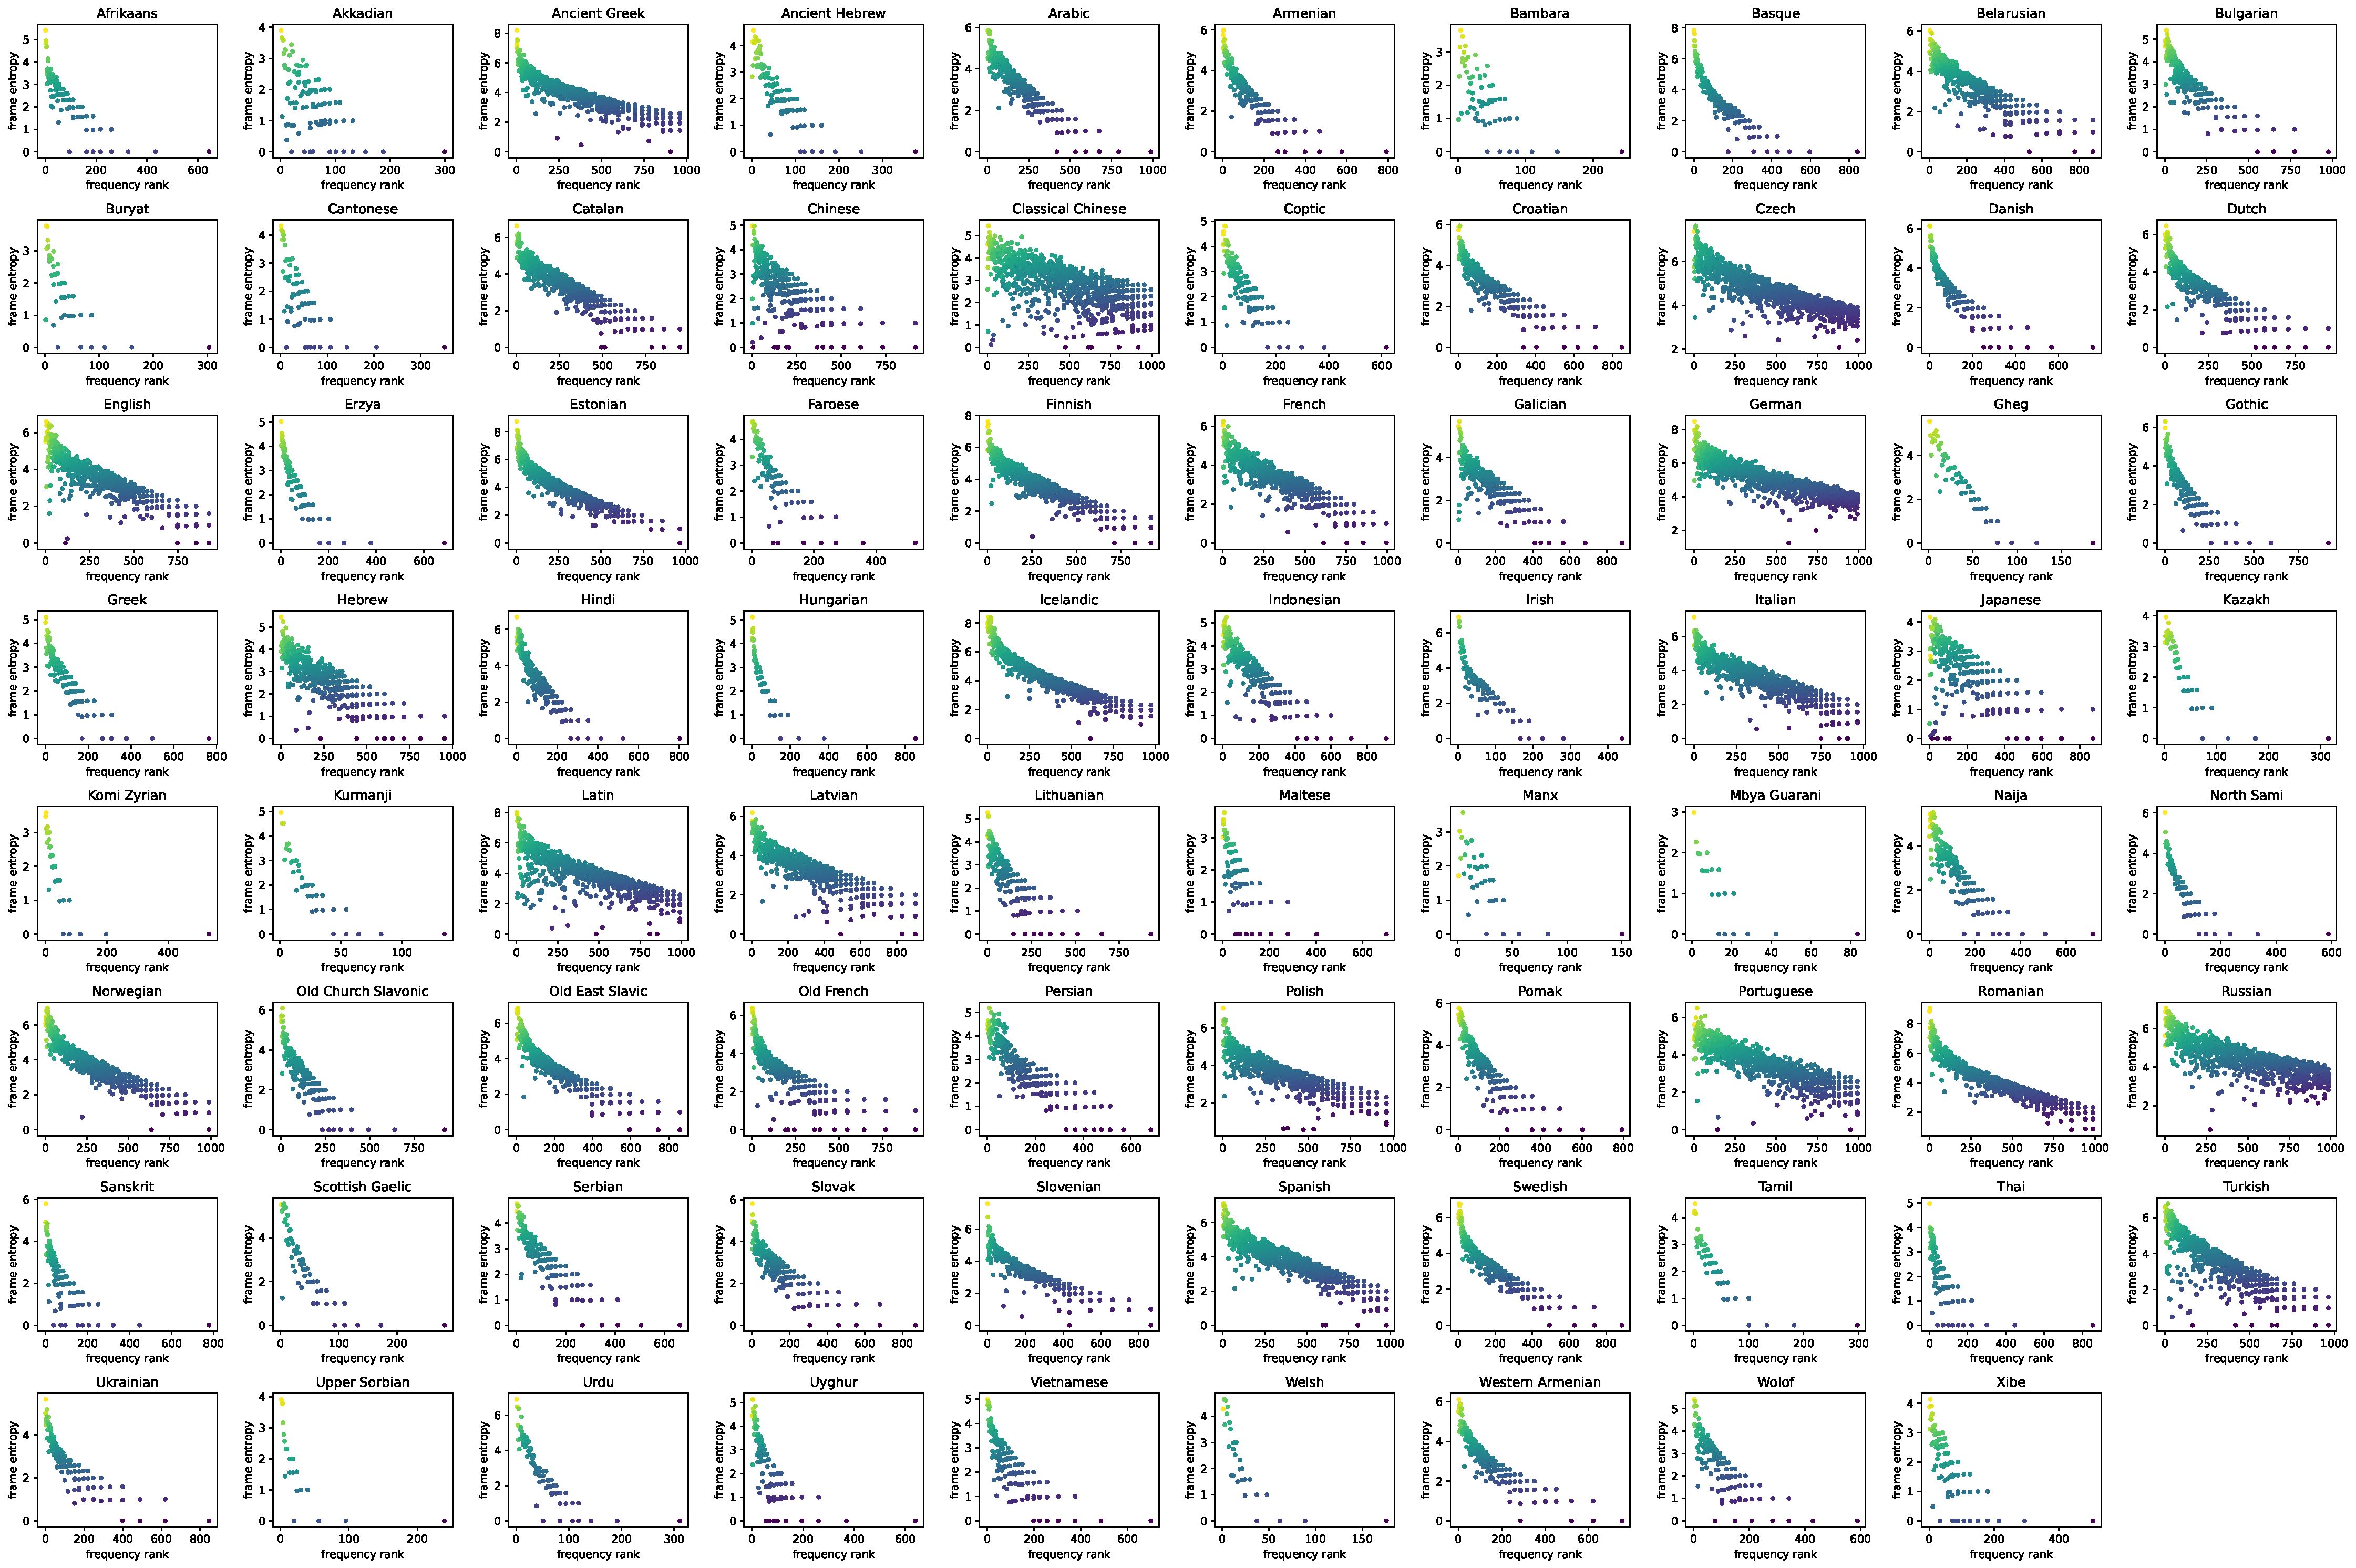
\includegraphics[width=\textwidth]{figures/joint_entropy_freq.pdf}
  \caption{Scatter plots showing relationship between valency frame entropy and frequency rank of verbs, color shows number of frames associated with the verb}
  \label{fig:joint_entropy_freq}
\end{sidewaysfigure}

\subsection{Analysis}

\section{Experiment 3: Ablation study of word order and case information}
\subsection{Experiment setup}
\subsection{Results}
\subsection{Analysis}

\section{Experiment 4: Frequency correlation with verbal entropy}
\subsection{Experiment setup}
\subsection{Results}
\subsection{Analysis}